\section{Introdução}

% Uma forma muito comum de acionamento de motores de corrente continua (CC) é por meio da modulação por largura de pulso, ou do inglês Pulse Width Modulation (PWM), que consiste basicamente em manipular a tensão média de alimentação do motor por meio de sinais digitais. É comum em certas aplicações o uso do sinal \emph{PWM} para manipular a velocidade do motor, ou seja, um controle de malha aberta, esse tipo de sistema apenas regula o quão rápido o motor irá girar. Porém na maioria das aplicações o controle em malha aberta não é suficiente, como por exemplo, não há garantias que se aplicadas tensões iguais (\emph{PWM}) em ambos os motores de um robô com acionamento diferencial (robôs com duas rodas tracionadas e independentes) o movimento será estritamente linear \cite{simple_speed_feedback}, isso é devido às diferenças entre os dois conjuntos de motores/rodas que fazem com que esses não girem a uma mesma velocidade, mesmo sobre uma mesma tensão.\\

% Existem diversos desafios no projeto de robôs pequenos, além da questão mecânica, o tamanho reduzido também restringe a possibilidade de se usar \emph{Hardwares} com mais capacidade computacional, além dos tipos e a quantidade de sensores que podem ser usados. Robôs como os da equipe Poti de Futebol de robôs (do Departamento de Computação e Automação (DCA) da UFRN), que são voltados para a participação na \emph{Latin American Robotic Competition} (LARC) na categoria \emph{IEEE Very Small Size Soccer} (VSSS), têm dificuldades para conseguirem comportar um \emph{Hardware} capaz de executar um controle digital de velocidade para ambos os motores, além de possuírem sensores com uma baixa acurácia, dificultando assim o bom desempenho do sistema de controle.\\

% O objetivo geral deste trabalho é projetar um sistema que realize o controle de velocidade dos motores de um robô com acionamento diferencial e que utiliza um estimador de velocidade sobre medições feitas com \emph{Encoders} de baixa resolução. Para a validação do trabalho foi feito a implementação do sistema proposto, testado em robôs reais e feito análises da eficiência dos controladores com relação à diminuição das assimetrias dos conjuntos motor-roda, bem como a qualidade da filtragem/estimativa da velocidade.

\begin{frame}{Motivação}
    \begin{figure}[H]
        \begin{subfigure}{.5\textwidth}
        \centering
        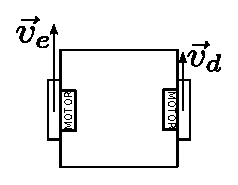
\includegraphics[width=0.5\textwidth]{figuras/ilustracoes/ilustracao_robo_diferentes_velocidades.eps}
        \end{subfigure}
        \begin{subfigure}{.5\textwidth}
        \centering
        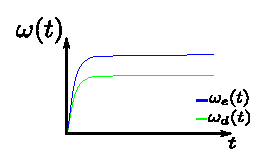
\includegraphics[width=\textwidth]{figuras/ilustracoes/ilustracao_caso_motivacional.eps}
        \end{subfigure}
        \caption{Ilustração. Respostas diferentes para uma mesma tensão de entrada nos motores direito e esquerdo.}
    \end{figure}
\end{frame}

\begin{frame}{Motivação}
Sensores com baixa resolução.
    \begin{figure}[H]
        \centering
        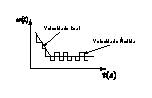
\includegraphics[width=0.7\textwidth]{figuras/ilustracoes/ilustracao_erro_de_quantizacao.eps}
        \caption{Ilustração do erro de quantização na medição da velocidade do motor.}
    \end{figure}
\end{frame}

\begin{frame}{Objetivos}
    \begin{itemize}
        \item Implementar um sistema de controle embarcado para os mini robôs da Equipe POTI de futebol de robôs do DCA;
        \item Utilizar um estimador de velocidade para reduzir o erro de quantização dos sensores.
    \end{itemize}
\end{frame}

\begin{frame}{Objetivos}

\begin{itemize}
    \item Esquema de Controle: \emph{FeedForward} + Controlador Proporcional;
    \item Filtro de \emph{Kalman} como estimador de velocidade.
\end{itemize}

\begin{figure}[H]
    \centering
    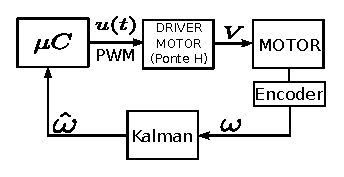
\includegraphics[width=0.5\textwidth]{figuras/ilustracoes/sistema_de_controle_embarcado.eps}
    \caption{Diagrama simplificado do sistema de controle embarcado para um motor.}
\end{figure}

\end{frame}